\documentclass[11pt]{exam}

\usepackage{amsmath, amssymb, multicol}
\usepackage{graphicx}
\usepackage{textcomp}
\usepackage{chessboard}
\usepackage{tikz}

\def\d{\displaystyle}
\def\b{\mathbf}
\def\R{\mathbf{R}}
\def\Z{\mathbf{Z}}
\def\st{~:~}
\def\bar{\overline}
\def\inv{^{-1}}


%\pointname{pts}
\pointsinmargin
\marginpointname{pts}
\addpoints
\pagestyle{head}
%\printanswers

\firstpageheader{Math 228}{\bf Towers and Tiles}{Wednesday, September 27}


\begin{document}

%space for name
%\noindent {\large\bf Name:} \underline{\hspace{2.5in}}
%\vskip 1em

\subsection*{Activity 1: Tower of Hanoi}

As the legend goes, there is a monastery in Hanoi with a great hall containing 3 tall pillars.  Resting on the first pillar are 64 giant disks (washers), all different sizes, stacked from largest to smallest.  The monks are charged with the following task: they must move the entire stack of disks to the third pillar.  However, due to the size of the disks, the monks cannot move more than one at a time.  And because the disks are so heavy and fragile, the monks may never place a larger disk on top of a smaller disk.

When the monks finally complete their task, the world shall come to an end.  Your task: figure out how long before we need to start worrying about the end of the world.

\begin{questions}
  \question This seems like a really hard counting problem.  So work on an easier one.  Find the minimum number of moves required for a smaller number of disks.  Collect some data. Make a table.

  \begin{solution}
  Just by moving the disks around, we can find the minimum number of moves for a small number of disks:

  \begin{center}
  \begin{tabular}{l|c|c|c|c}
  Number of disks: & 1 & 2 & 3 & 4 \\ \hline
  Min Number of moves: & 1 & 3 & 7 & 15
  \end{tabular}
  \end{center}
  \end{solution}
  \vfill
  \question Conjecture a formula for the minimum number of moves required to move $n$ disks.  Test your conjecture.  How do you know your formula is correct?
  \begin{solution}
	  The numbers in the sequence so far are all one less than a power of 2.  So a reasonable conjecture would be $a_n = 2^n - 1$.  Notice that this is a \emph{closed} formula and it is not obvious it is correct.  If all we ask for is a \emph{recursive} formula, we notice right away that $a_n = 2a_{n-1} + 1$, since to move $n$ disks, we can move $n-1$ disks to a peg, move the last disk, then move the $n-1$ smallest disks back on top of the last disk.
  \end{solution}

  \vfill
  \question If the monks were able to move one disk every second without ever stopping, how long before the world ends?

  \begin{solution}
	  $2^{64}-1$ seconds is roughly 580 billion years.
  \end{solution}

  \vfill

\end{questions}


\newpage

\subsection*{Activity 2: Counting Strips}

You have a large collection of tiles: $1\times 1$ squares and $1\times 2$ dominoes.  You want to arrange these to make a $1 \times 15$ strip.  How many ways can you do this?

For example, here are a few different $1\times 4$ strips:
\vskip 1ex
\centerline{
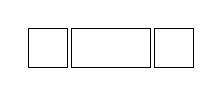
\begin{tikzpicture}[scale=.5]
  \draw (0,0) rectangle (1,1) (1.1,0) rectangle (3.1,1) (3.2,0) rectangle (4.2,1);
\end{tikzpicture}
\hspace{.5in}
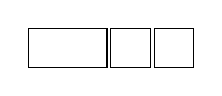
\begin{tikzpicture}[scale=.5]
  \draw (0,0) rectangle (2,1) (2.1,0) rectangle (3.1,1) (3.2,0) rectangle (4.2,1);
\end{tikzpicture}
\hspace{.5in}
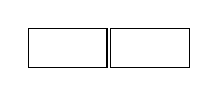
\begin{tikzpicture}[scale=.5]
  \draw (0,0) rectangle (2,1) (2.1,0) rectangle (4.1,1);
\end{tikzpicture}
}


\begin{questions}
  \question Again, start by collecting data: How many length $1\times 1$ strips can you make?  How many $1\times 2$ strips?  How many $1\times 3$ strips?  And so on.
  \begin{solution}
  There is only one $1\times 1$ strip.  There are two $1\times 2$ strips (SS, D).  There are three $1\times 3$ strips (SSS, DS, SD).  Here is a table of this data:

  \begin{center}
  \begin{tabular}{l|c|c|c|c|c}
  $n$ & 1 & 2 & 3 & 4 & 5 \\ \hline
  $1\times n$ strips: & 1 & 2 & 3 & 5 & 8
  \end{tabular}
  \end{center}
  \end{solution}
  \vfill
  \question How are the $1\times 3$ and $1 \times 4$ strips related to the $1\times 5$ strips?  Hint: consider two cases, the strips that start with a square and strips that start with a domino.
  \begin{solution}
  Each $1\times 5$ strips either starts with a square or a domino.  If it starts with a square, then the square is followed by one of the five $1 \times 4$ strips.  If it starts with a domino, it is followed by one of the three $1 \times 3$ strips.  Thus the number of $1\times 5$ strips is equal to the number of $1\times 3$ strips plus the number of $1 \times 4$ strips.
  \end{solution}

  \vfill
  \question How many $1\times 15$ strips can you make?
  \begin{solution}
	  Following the patter above, we extend the table to get up to 15:
	    \begin{center}
	    \begin{tabular}{l|c|c|c|c|c|c|c|c|c|c|c}
	    $n$ & 5 & 6 & 7 & 8 & 9 & 10 & 11 & 12 & 13 & 14 & 15 \\ \hline
	    $1\times n$ strips: & 8 & 13 & 21 & 34 & 55 & 89 & 144 & 233 & 377 & 610 & 987
	    \end{tabular}
	    \end{center}
  \end{solution}
  \vfill
  \vfill
  \question What if I asked you to find the number of $1\times 1000$ strips?  Would the method you used to calculate the number of  $1 \times 15$ strips be helpful?

  \begin{solution}
  No, we would need to compute the table all the way up to 1000 (not too difficult with a computer, but not something we want to do by hand).  This is because we only have a \emph{recursive} definition for the sequence, not a closed formula.
  \end{solution}
%  \question Can you see a relationship between the number of length 3 paths, the number of length 4 paths, and the number of length 5 paths?  Does this relationship work for length 4, 5, and 6 paths as well?  Use this to find the number of length 10 paths.
%  \vfill
%  \question Does the relationship you found in part 2 always hold?  Why?
%  \vfill
%  \question If you were to build all possible length 1 paths, all possible length 2 paths, and so on up to all possible length $5$, how many paths will you have total?  What if you go up to all paths of length $n$?
%  \vfill
\end{questions}



\end{document}
